\documentclass[a4paper]{report}
\usepackage[english]{babel}
\usepackage{amsfonts}
\usepackage{amsmath} % Equation numbering
\usepackage[square,sort,comma,numbers]{natbib}

\usepackage{graphicx} % Figures
\usepackage{grffile} % For recognising the png-extension
\usepackage{float} % For floating figures

\usepackage{changes} % For track changed extensions
\usepackage{todonotes}

\usepackage{dsfont} % For indicator function

\usepackage{hyperref}
\bibliographystyle{plainnat}

% For example environment
\usepackage{amsthm}
\theoremstyle{definition}
\newtheorem{example}{Example}[section]

% For theorem environment
\newtheorem{theorem}{Theorem}
\begin{document}
\section{Trace Lifetime Analysis}
To be able to predict the remaining time until a failure, it is helpful to know how the lifetime of the traces is distributed. In this section we will attempt to fit the lifetime of the traces to a distribution.

\subsection{Normality}
The first guess for a fitting distribution would be a normal distribution. However, the Shapiro-Wilk normality test rejected the hypothesis that the lifetimes are normally distributed with a p-value of $1.26\times 10^{-5}$. Hence, we can safely conclude that the data do not follow a normal distribution. This is also visible on the following quantile-quantile plot.
\begin{figure}[H]
\centering
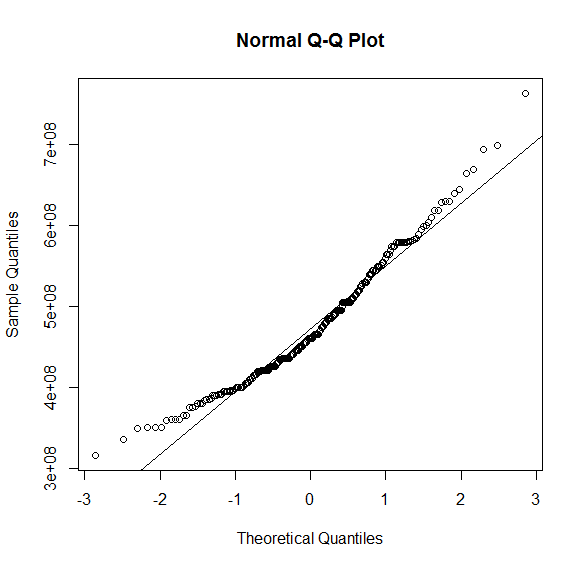
\includegraphics[width=0.8\textwidth]{Plots/QQPlot.png}
\caption{Quantile-quantile plot of the trace lifetimes.}
\end{figure}

\subsection{Cullen and Frey graph}
\begin{figure}[H]
\centering
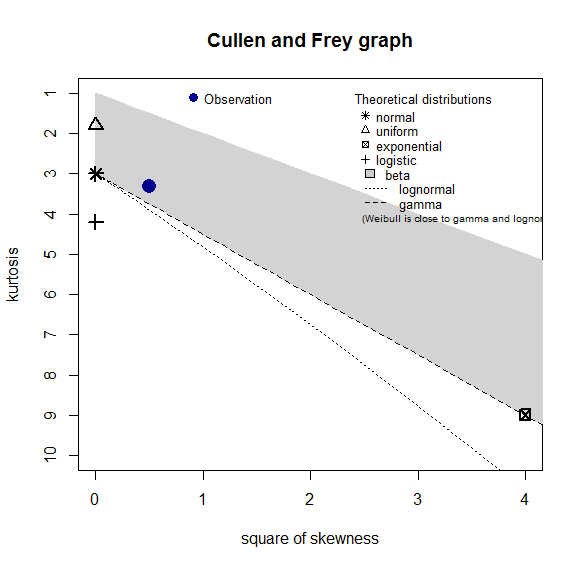
\includegraphics[width=0.8\textwidth]{Plots/CullenAndFray.png}
\caption{Cullen and Fray graph of the data.}
\end{figure}
Above, a Cullen and Fray graph is plotted. The data is placed based on its kurtosis and skewness. A few well-known distributions are also plotted on this plane. This plot would suggest a beta distribution. However, the beta distribution has a support of $[0,1]$ while the lifetime of a trace is not bounded. Other distributions that have similar kurtosis and skewness are the Weibull distribution and the gamma distribution.


\bibliography{bibliography}

\end{document}